\documentclass[thesis,fonts=libertine]{cluu}

\usepackage[style=cluu]{biblatex}
\usepackage{amsmath}

\DeclareMathOperator*{\argmax}{arg\,max}
\DeclareMathOperator*{\argmin}{arg\,min}

\usepackage{tikz}
\usepackage{graphicx}
\usepackage{url}
\usepackage{listings}
\usepackage{siunitx}
\usepackage[boxed, noline]{algorithm2e}

\graphicspath{ {figures/} }
\addbibresource{thesis.bib}

\usepackage{pythonhighlight}    % for \inputpython at the end

\begin{document}
\author{Shifei Chen}
\supervisors{Ali Basirat, Uppsala University}
\title{When and Why Universal Word Embeddings Are Not Useful in a Zero-Shot Machine Translation System}

\maketitle

\begin{abstract}
  The concept of \emph{palindromes} is introduced, and some method for
  finding palindromes is developed.
\end{abstract}

\tableofcontents

\addchap{Preface}

This thesis was finished under the supervision from Ali Basirat. I would like 
to thank him for his continuous help and inspriration.

I would like to thank Mr. Anders Wall and everyone in the Anders Wall Scholarship Foundation for sponsoring my Master study. I would also like to thank everyone in the Master Programme in Language Technology, including all of my classmates and the teachers. I have learned a lot from you during this 2-years journey.

Last but not least, I would like to say thank you to my parents for their unconditional love and support. Also to my girlfriend, who has always been together with me during this unusual time.

% by using \addchap instead of \chapter this preface isn't numbered.

\chapter{Introduction}

Palindromes are fun. I've tried to find some.
In Chapter \ref{chap:prev} previous work is reviewed, and
Chapter \ref{chap:results} is about my results.

\chapter{Previous work}
\label{chap:prev}

\section{Word Embeddings}
\subsection{Representing Words in Vectors}

In Natural Language Processing, people need to convert the natural representation of words into form that are more effieicent for computer to process. The idea started with statistical language modelling \parencite{bengio2003neural}. In 2013, \cite{Mikolov:2013aa} introudced Word2Vec, which encapsules words and their latent information into vectors. Besides the benefit that it simplifies representation and storage of words for computers, it also enables the possibilities to calcualte word and their semantic meanings just as vectors.

Take an example vocabulary $V=\{\text{king}, \text{queen}, \text{man}, \text{woman}\}$, if we convert these words into vectors such as 

\begin{align*}
  \vec{k} &= \text{vec}(\text{king})\\
  \vec{q} &= \text{vec}(\text{queen})\\
  \vec{m} &= \text{vec}(\text{man})\\
  \vec{w} &= \text{vec}(\text{woman})
\end{align*}

We could have an equation of 

\begin{equation}
  \label{equa:semantic_vectors}
  \vec{q}=\vec{k}-\vec{m}+\vec{w}
\end{equation}

It is meaningful from both the mathmatical prospective and the linguistic prospective. The latter can be illustrated by Figure \ref{fig:semantic_vectors} in a vector space that contains these four vectors. In addition, the two cosine similarity values of vectors $\vec{k}$ and $\vec{q}$, and of $\vec{m}$ and $\vec{w}$ should also be close, as the angles between each two vectors are about the same.

\begin{figure}
  \centering
  \tikzset{every picture/.style={line width=0.75pt}} %set default line width to 0.75pt
  \begin{tikzpicture}[x=0.75pt,y=0.75pt,yscale=-1,xscale=1]
    %uncomment if require: \path (0,256); %set diagram left start at 0, and has height of 256

    %Shape: Axis 2D [id:dp40983147480798976]
    \draw  (49,221.35) -- (260.5,221.35)(70.15,31) -- (70.15,242.5) (253.5,216.35) -- (260.5,221.35) -- (253.5,226.35) (65.15,38) -- (70.15,31) -- (75.15,38)  ;
    %Straight Lines [id:da3468248594605029]
    \draw [color={rgb, 255:red, 74; green, 144; blue, 226 }  ,draw opacity=1 ]   (70.15,221.35) -- (91.04,133.95) ;
    \draw [shift={(91.5,132)}, rotate = 463.44] [color={rgb, 255:red, 74; green, 144; blue, 226 }  ,draw opacity=1 ][line width=0.75]    (10.93,-3.29) .. controls (6.95,-1.4) and (3.31,-0.3) .. (0,0) .. controls (3.31,0.3) and (6.95,1.4) .. (10.93,3.29)   ;
    %Straight Lines [id:da060011766798584776]
    \draw [color={rgb, 255:red, 80; green, 227; blue, 194 }  ,draw opacity=1 ][fill={rgb, 255:red, 182; green, 34; blue, 34 }  ,fill opacity=1 ]   (70.15,221.35) -- (98.61,163.79) ;
    \draw [shift={(99.5,162)}, rotate = 476.31] [color={rgb, 255:red, 80; green, 227; blue, 194 }  ,draw opacity=1 ][line width=0.75]    (10.93,-3.29) .. controls (6.95,-1.4) and (3.31,-0.3) .. (0,0) .. controls (3.31,0.3) and (6.95,1.4) .. (10.93,3.29)   ;
    %Straight Lines [id:da268618270283273]
    \draw [color={rgb, 255:red, 208; green, 2; blue, 27 }  ,draw opacity=1 ]   (70.15,221.35) -- (127.85,182.12) ;
    \draw [shift={(129.5,181)}, rotate = 505.79] [color={rgb, 255:red, 208; green, 2; blue, 27 }  ,draw opacity=1 ][line width=0.75]    (10.93,-3.29) .. controls (6.95,-1.4) and (3.31,-0.3) .. (0,0) .. controls (3.31,0.3) and (6.95,1.4) .. (10.93,3.29)   ;
    %Straight Lines [id:da46956564149919644]
    \draw [color={rgb, 255:red, 245; green, 166; blue, 35 }  ,draw opacity=1 ]   (70.15,221.35) -- (131.69,192.84) ;
    \draw [shift={(133.5,192)}, rotate = 515.14] [color={rgb, 255:red, 245; green, 166; blue, 35 }  ,draw opacity=1 ][line width=0.75]    (10.93,-3.29) .. controls (6.95,-1.4) and (3.31,-0.3) .. (0,0) .. controls (3.31,0.3) and (6.95,1.4) .. (10.93,3.29)   ;

    % Text Node
    \draw (83,108) node [anchor=north west][inner sep=0.75pt]   [align=left] {$\vec{k}$};
    % Text Node
    \draw (101,142) node [anchor=north west][inner sep=0.75pt]   [align=left] {$\vec{q}$};
    % Text Node
    \draw (132,166) node [anchor=north west][inner sep=0.75pt]   [align=left] {$\vec{m}$};
    % Text Node
    \draw (138,183) node [anchor=north west][inner sep=0.75pt]   [align=left] {$\vec{w}$};
  \end{tikzpicture}
  \caption{Illustraion of a vector space where Equation \ref{equa:semantic_vectors} exists.}
  \label{fig:semantic_vectors}
\end{figure}

To turn words into vectors, one could use simple one-hot encoding. Like in the example above we could make $\vec{k}=[1, 0, 0, 0]$. But these one-hot vectors can merely capture any latent semantic meanings between different words. Recent vectorized word representations, or word embeddings, were learned through neural networks, such as Word2Vec which learns word embeddings through a Skip-gram model or a Continuous Bag of Words model \parencite{Mikolov:2013ab}.

\subsubsection{The Skip-gram model}

When given a target word $w$, the model can produce vector representations that are good at predicting the words surrounding $w$ within the context size of $C$. The probability of a context word $w_k$ given a target word $w$ is:

\begin{equation}
  P(w_k|w)=\frac{\exp({v_{w_k}^\prime}^\intercal v_w)}{\sum_{i=1}^{|V|}\exp({v^\prime_i}^\intercal v_w)}
\end{equation}

Here $|V|$ means the size of the whole vocabluary from the corpus, $v^\prime$ and $v$ stand for the vector representation of the input and the output vector representation of a word \parencite{Mikolov:2013aa}. The input representation $v^\prime$ could be initialized by one-hot representations.

\subsubsection{The Continuous Bag of Words model (CBOW)}

The other model, CBOW, works just as the other side the coin. It predicts the target word $w$ based on a bunch of context words $w_{-C}, w_{-C+1} ..., w_{C-1}, w_C$ within the window size $C$, as the formula below:

\begin{equation}
  P(w|w_{-C}, w_{-C+1} ..., w_{C-1}, w_C)=\frac{\exp({v^\prime_w}^\intercal \bar{v}_{w_k})}{\sum^{|V|}_{i=1}\exp({v^\prime_{w_i}}^\intercal \bar{v}_{w_k})}
\end{equation}

Here $\bar{v}_{w_k}$ means the sum of the context word $w_k$'s vectorized representation, while $v^\prime_w$ means the input vector representations of word $w$ as in the Skip-gram model. 

The difference between these two models is that the CBOW model predicts the target word from multiple given context words, while the Skip-gram model predicts the context words from one given center word. Hence the skip-gram model is better at predicting rare words because all of the words are treated equally in the \textit{word AND context} relationship. But in the CBOW model, common words have advantages over rare words as they will have higher probability in a given context. The Skip-gram model is arguably the most popular method to learn word embeddings as it is both fast and robust \parencite{levy-etal-2015-improving}.

\subsection{Cross-Lingual Word Embeddings}

Vectorized word representations tends to cluster words that are semantically similar to each other. It then become very attractive to see whether we could fit two or more langauges into the same vector space. This is so called multilingual word embeddings.

\begin{figure}
  \label{fig:vec_space_align}
  \centering
  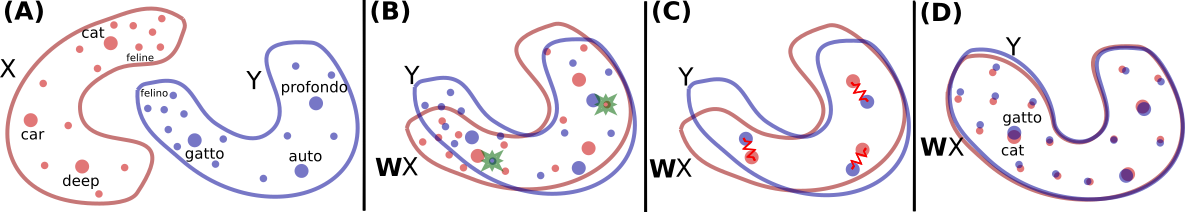
\includegraphics[width=0.8\textwidth]{vector_spaces_alignment.png}
  \caption{Aligning bilingual vector spaces. \parencite{Conneau:2017aa}}
\end{figure}

In such case, it is then vital to align words in two different vector spaces. As show in Fig. \ref{fig:vec_space_align}, which illustrated the alignment method from \cite{Conneau:2017aa}. Suppose there is a set of word pairs in their associated vertorized representation $\{x_i, y_i\}_{i\in \{1, ..., n\}}$, the two vector spaces were aligned by learing a rotation matrix $W \in \mathbb{R}^{d \times d}$ as in process \textbf{(B)}, where we try to optimize the the formula 

\begin{equation}
  \min_{W \in \mathbb{R}^{d \times d}} \frac{1}{n}\sum_{i=1}^n \ell(Wx_i, y_i)
\end{equation}

. Here $\ell$ is the loss function and it is usually the square loss funciton $\ell_2(x, y)=||x-y||^2$. $W$ is then further refined in process \textbf{(C)}, where frequent words were selected as anchor points and the distance between each corrospondent anchor points were minimized by using an energy function. After this, the refined $W$ is then used to map all words in the dictionary during the inference process. The translation $t(i)$ of a given source word $i$ is obtained in the formula

\begin{equation}
  t(i) \in \argmin_{j\in \{1, ..., N\}} \ell(Wx_i, y_j)
\end{equation}

. Again, the loss function $\ell$ is typically the square loss function. However using square loss could make the model suffer from the ``hubness problem''. \cite{Conneau:2017aa} counter reacted to the ``hubness'' problem by introducing the cross-domain similarity localscaling (CSLS).

The initial alignment data to for adversarial learning the rotation matrix $W$ could come from a bilingual dictionary \parencite{Mikolov:2013ac}. There are other kinds of alignment by using aligned data from sentence level, or even document level. By using word-level information, we can start with a pivot lanugage (usually English) and map each other monolingual word embeddings by looking up translation dictionaries. This could also be done starting with bilingual vector spaces, where we choose a bilingual word embedding that shares a language (typically English) with other bilingual embeddings, and choose other bilingual word embeddings by aligning their shared language subspace. Sentence-level parallel data are similar data as the corpus in Machine Translation (MT), which contains sentence-aligned texts \parencite{Hermann:2013aa}. Document-level information are more common in the form of topic-aligned or class-aligned, such as Wikipedia data \parencite{vulic-moens-2013-study}.

The alignment process of multilingual word embeddings are roughly the same as bilingual word embeddings, using parallel data from either word-level, sentence-level or document-level \parencite{Ruder:2019aa}.

\subsection{fastText}

In this work, we have chosen fastText aligned word vectors \footnote{\url{https://fasttext.cc/docs/en/aligned-vectors.html}} \parencite{Joulin:2018aa} as our vectorized word representation. They are based on the pre-trained vectors computed on Wikipedia using fastText \parencite{Bojanowski:2016aa}.

fastText is an extension to the original Word2Vec methods which uses sub-words to augment low-frequency and unseen words. For example, \texttt{low-key} as a whole word its possibility in a given document would be much lower than each of the component, \texttt{low} and \texttt{key}. fastText learns its vectorized representation from a smaller n-gram sub-word level. It divides the whole word into sub-words units as below if we assume $n=3$

\begin{equation*}
  \mathtt{\text{<}lo, low, ow\text{-}, w\text{-}k, \text{-}ke, key, ey\text{>}}
\end{equation*}

Each of the sub-word has its own vectorized representation learned through a CBOW or Skip-gram model as in Word2Vec. The word vector for the whole word unit \texttt{<low-key>} is then the sum of all of its sub-word units' vectors, hence its rareness would be compensated by two rather frequent subwords \texttt{low} and \texttt{key}, even if it might not appear in the training document at all.

In terms of multilingual alignement, fastText improves the common solution to the hubness problem by directly including the Relaxed CSLS (RCSLS) criterion into the model during both the learning and the inference phrase. Before the work of \cite{Joulin:2018aa}, inverted softmax (ISF) \cite{Smith:2017aa} or CSLS \parencite{Conneau:2017aa} was only used in the inference time to address the hubness problem while square loss is still the loss function used in the training time. But since both the ISF and the CSLS are not consistent with the square loss function in the training time, they will create a discrepancy between the learning of the translation model and the inference.

\section{Multilingual Neural Machine Translation (MNMT) Systems}

\subsection{Multilingual Machine Translation}

\subsection{Zero-shot Machine Translation Systems}

Zero-shot translation stands for transltion between language pairs that are invisible for the MNMT system during the training time. E.g., we build a MNMT system with training language pairs of German-English and French-English while test its performance on a German-French scenario. In 2016, \cite{Johnson:2016aa} first published their result on a zero-shot MT system. Their multilingual MT system, which includes a encoder, decoder and attention module requires no change to a standard NMT system. The only modification is in the training corpus, where they had introduced an artifitial token in the beginning of each source sentence to denote the target language to be tranlsated into. \cite{Ha:2016aa} also showed that their universal encoder and decoder model is capable to zero-shot MT. The concept of translation between unseen language pairs are attractive, especailly for low-resource language pairs, though these two models both underperformed than a pivot based system.

There are two reasons that could explain the gap between a zero-shot system and a pivot based system, language bias \parencite{Ha:2016aa,Ha:2017aa,Arivazhagan:2019aa} and poor generalization \parencite{Arivazhagan:2019aa}. Language bias means that during inference, the MT system has a tendency to decode the target sentence into the wrong language, usually copying the soruce language or the bridging language \cite{Ha:2016aa}. It could be the consequnce of always translating all source languages into the bridging language, hence make the model difficult to learn to translate the desired target language \parencite{Arivazhagan:2019aa}.

The other potential reason for the worse performance of a zero-shot system is poor generalization \parencite{Arivazhagan:2019aa}. When a zero-shot system is trained purely on the end-toend translation objective, the model prefers to overfit the supervised translation direction features than learn more transferable language features.

To fix these two problems, there has been work on improving the preprocessing process \parencite{Lakew:2018aa}, parameter sharing \parencite{Firat:2016aa, Blackwood:2018aa}, additional loss penalty functions \parencite{Arivazhagan:2019aa} and pre-training modules using external information \parencite{Baziotis:2020aa}. In some cases, zero-shot system could achieve better performance than pivot based systems.

\subsection{MNMT Systems Based on Word Embeddings}

One of the potential application of word embeddings is machine translation. In cases where people need to translate from or into a low-resource langauge, they usually find it difficult to locate enough parallel data that consists of such kind of less common language. If we could build up a vector space with word embeddings from different languages that are aligned, we could leverage the similarity of word embeddings to compensate the lack of parallel data \parencite{zou-etal-2013-bilingual}. We could find words that are never seen in the training data buy looking for their neighbours in the vector space. There are case where successfully trained a machine translation system using very little or none parallel data \parencite{Conneau:2017aa}.

There are successful applications of pre-trained word embeddings in a MT system, such as the embedding layer in an MT system \parencite{neishi-etal-2017-bag, Artetxe:2017aa}, the subsitution of a supervised dictionary \parencite{Conneau:2017aa}, or an external supplementary extension \cite{inproceedings}. But in most MT systems, using pre-trained word embeddings purely as the embedding layer will not outperform other models such as Transformers \parencite{Vaswani:2017aa} and its other evolutions, largely because the training data for a MT system is usually several orders of magnitude larger than the monolingual pre-trained word embeddings. Typically pre-trained word embeddings are mainly introduced in MT systems dealing with low-resource languages.

For NMT system focused in low resource language, \cite{Qi:2018aa} looked into the question of when and why are pre-trained word embeddings useful. They found that pre-trained word embeddings are consistantly useful for all languages, the gains would be more visible if the source and target language are similar, such as langauges within the same family. Also, pre-trained word embeddings need to be applied on a MT system with at least a moderate performance. In other words, pre-trained word embeddings can not work when there is not enough data to train a basic MT system. Finally, aligned word embeddings is useful in a multilingual MT system. For bilingual MT systems, pre-trained word embeddings don't necessarily need to be aligned.

Moreover, aligned word embeddings doesn't work well for moporlogically rich languages such as Russian and Belarusian. \cite{Qi:2018aa} argue that this may mainly due to the sparsity in the word embeddings files. In addition, most of the previous works are target on zero-shot language pairs, not on compeletely unseen languages. For language pairs $A \rightarrow \text{EN}$ and $\text{EN} \rightarrow B$, they are all interested in the unseen language pair $A \rightarrow B$. For language pairs that includes an unseen language $C$, whether it is in the source side or the target side, it remains to be seen how universal word embeddings could help translate in this scenario.

\chapter{Error Analysis in a Word Embedding Based MNMT System}
\label{chap:error_analysis}

In this chapter I will perform experiments in a universal word embedding based MNMT system. Then I will analysis its results to show why such kind of system failed to translation compeletly unseen languages depite its theoratical feasibility.

\section{Theoratical Feasibility}

As mentioned in Chapter \ref{chap:prev}, \cite{Mikolov:2013ac} showed that there is a linear relationship between similar word embeddings in different languages. For each word pairs, assume their vector representations are $\{x_i, y_i\}_{i=1}^n$, we could calcualte a transformation matrix $W$ such that $Wx_i$ approximates to $y_i$. \cite{Mikolov:2013ac} also showed their result in the word/phrase translation task for suck kind of approximated word embedding mappings. For some subsets of words, around 70\% of word embeddings are exactly matched with each other by calcluating the Precision@5 score. If the threshold for the cosine similarity $\max\cos(Wx, y_i)$ being loosed to 0.6, the Precision@5 score would be as high as 90\%.

In order to convert words into vectors to be calculated in the neural network, NMT systems should treat each word as word embeddings. The value of these word embedding could be learned directly during translation, but then the initialization is a crucial step as poor initialization could lead to slow converge or worse local mimima \parencite{glorot2010understanding}. The situation could be even more challenging when transltion with very few parallel corpora, since there is no data to help the embedding layer to converge to its ideal state. Hence the aforementioned word embedding mapping technique becomes appealing.

\cite{Qi:2018aa} explored how effective it is by using aligned pre-trained word embeddings in a NMT system. They found that regardless of languages, alignment is useful as long as it's applied in a multilingual setting. They believe that since both the source and the target side vector spaces are already aligned, the NMT system learns how to transform the simialr fashion from the source langauge to the target language.

Therefore, translating a compeletely unseen language can be viewed as the question below --- Given a vector space $Z$ that consists of aligned word embeddings $\{a_i, b_i, c_i, ...\}$, how much does the NMT system knows about an unseen language $A$ if it was only trained on the remaining languages? In theory, since the word embeddings are clustered by their semantic meanings in the vector space $Z$, we should be able to build loose mappings between each of the semantic centers from both the source side and the target side. The generalization ability of the system is the key to answer this question. Hence I conducted some prelimentary experiments below.

\section{Experiment Settings}

To get a basic multilingual MT system running, I chose English (EN), Germen (De) and French (FR) to be my training languages. Let $C$ donate the final corpus, $l$ donates the langauge specific corpus fragment and $Z$ is the set of correspoding candidate langauges, $Z_{TRAIN} = {l_{EN}, l_{DE}, l_{FR}}$. I picked up Swedish (SV), Hungarian (HU) and Hebrew (HE) being my test languages, therefore $Z_{TEST} = {l_{SV}, l_{HU}, l_{HE}}$.

For each experiment, a basic MNMT system is trained using a training corpus  $C_{TEST}$ with all three training languages , including all six directions from the cartesian product without duplicates

\begin{equation}
  C_{\text{TRAIN}} = \{x \times y \mid x, y \in Z_{\text{TRAIN}} \text{ and } x \neq y\}
\end{equation}

It is tested on the test corpus with all three training languages and one of the test language, consist of bidirections of three different training language to the only test language.

\begin{equation}
  C_{\text{TEST}} = \{(x, y)\cup(y,x) \mid x \in Z_{\text{TRAIN}} \text{ and } y \in Z_{\text{TEST}}\}
\end{equation}

I designed the experiments and picked up the training and target languages based on the following aspects.

\subsubsection{Language Similarity}

In the work \cite{Qi:2018aa} the authors mentioned their observation that pre-trained word embeddings are useful for languages from the same language family, the closer their relationship is the higher the performance improve is. For aligned word embeddings, if it is applied in a MNMT system consist of langauges from the same language family, it will also be benificial.

\subsubsection{Shared Alphabets}

In a typical word embedding based NMT system without subword encoding, it uses a word to index mapping to look up a correspoding word embedding for each word in the text, and a reverse index to word mappding to reconstruct the human readible text from its inferrencens. During the whole process, every word is treated as a whole, no subword segment is available. This is different than a Transformer system which subword encodings like BPE or sentencepiece are commonly used. Although fastText word embeddings were learned by using subword information \parencite{Bojanowski:2016aa}, in the final representation form all of the subword informatino is no longer available. Hence the NMT system could learn a rough mapping from semantics in the source language to the target language in a common vector space, it might see a big drop for distant languages that don't share a common alphabets.

\subsubsection{Word Order}

For a word embedding based NMT system, syntactic information lies compleetely in its hidden layer. This again differs from a Transformer system. Transformer systems learn both the lexicon, syntactic and semantic information all together in their hidden layers. Hence it remains to see how word embedding based MNMT performs on languages with different word orders, e.g. SVO versus SOV languages.

\subsection{Corpus and Preprocessing}

I used the TED talk subtitile corpus from \cite{Qi:2018aa} \footnote{\url{https://github.com/neulab/word-embeddings-for-nmt}} to train my NMT. The whole corpus has roughly 270000 sentences was splited into three parts, train, dev, test at the ratio of $0.95:0.025:0.025$.

To build up the corpus for each experiment, I have modified the original script from \cite{Qi:2018aa} and added a few customized features. In short, the script will extract the common sentence from each part of the splited corpus to form up a common intersection used in training, developing and testing. Since our experiments consists of languages that are relatively common in the TED project, this fine tuned corpus isn't too much different from the original corpus, hence the size for the train, dev and test split are still kept afterwards.

For preprocessing, since the orginal TED corpus is already tokenized by Moses, I then turned all of the text into lowercases and applied a sentence lengh filter to remove any long sentence that have more than 60 word to prevent bad perfromance in training. After that, when building the i2w and w2i index for the pre-trained embeddings, I have also remove any words that are less frequent than 2 times to stop the system from overfitting with too much low-frequency words. All of the preprocess function are built upon the built-in XNMT preprocess features \parencite{Neubig:2018aa}.

\subsection{Neural Network}

For the neural network I used a modified version of the neural network from \cite{Qi:2018aa}, which is built with XNMT \cite{Neubig:2018aa}. I have doubled the encoding layer to a 2-layer-bidirectional LSTM network and added the accuracy score as a evaluation metric alongside the BLEU score \parencite{papineni-etal-2002-bleu}. Everything else are kept from the orignal experiment settings, including a encoder-decoder model with attention \parencite{Bahdanau:2014aa} and a beam size of $5$, trained using batch of 32 and the Adam optimizer \parencite{Kingma:2014aa}. The initial learing starts at $0.0002$ and decays by $0.5$ when development BLEU score decreases \parencite{Denkowski:2017aa}.

\subsection{Embeddings}

The embeddings I used are fastText aligned word embeddings\footnote{\url{https://fasttext.cc/docs/en/aligned-vectors.html}}. They are based on the pre-trained vectors on Wikipedia\footnote{\url{https://www.wikipedia.org/}} using fastText \parencite{Bojanowski:2016aa}. The alignment is performed using RCSLS as in \cite{Joulin:2018aa}.

Each of the fastText word embedding file is language specific and contains word embeddings in 300 dimensions. I concatnated different language files To build up multilingual word embedding files for the MNMT system. If there is a shared word $w$ with two different vector values $\vec{v_a}$ and $\vec{v_b}$ in different embedding files, I will add those two vectors up and pick the average value $\vec{v_{mean}}$ as the new vector.

\begin{equation}
  \vec{v_{mean}} = \vec{v_a} + \vec{v_b} / 2
\end{equation}

In this way, there are possibilities that both of the unique semantic values in the two words $w_a$ and $w_b$ could lost, as there are cases that word with distant meaning share the same spelling in different languages. But it could also be argued that many word with the same spelling do have similar meaning. For example the word \verb|café| means the same thing in both English and French, as English borrowed that word from French. Later in the experiment I also tried a different approach where I treat each word as a unique word despite they might share the same spelling, both of the results are shown below.

\section{Results and Analysis}

Before I got the results, I anticipated that among all three test languages, Swedish will get the best result and it could be on the same level as the baseline MNMT consists of EN, DE and FR only. The other two languages will not get any close to the performance of Swedish, and they could go down to less than 10 BLEU scores.

\begin{table}
  \centering
  \begin{tabular}{c c c}
    cell1 & cell2 & cell3 \\ 
    cell4 & cell5 & cell6 \\  
    cell7 & cell8 & cell9 
  \end{tabular}
  \caption{Initial results for SV, HU and HE on the baseline system (Target language annotation only, dropout=0.3, trained on mixed language branch corpus.)}
  \label{table:initial_results}
\end{table}

However, in the results shown in Table \ref{table:initial_results}, all of the three languages got very low BLEU scores. Swedish, though it indeed was the best of three, only achieved about 3.5 BLEU score. The other two language, Hungarian and Hebrew, didnt even go abobe 1 BLEU score. The surprisingly low results made me curious and would like to check what could be improved.

\subsection{Altering the Source/Target Language Annotation}

The first improvement I tried is to alter the way the target langauge annotation in the source sentences. In the corpus building script I add a custom \verb|__{lang_id}__| token at the front of each source sentence as suggested in \cite{Johnson:2016aa}. A sentence in the processed source text that needs to be translated into German would look like 

\begin{verbatim}
  __de__ And we struggle with how to deal with them .
\end{verbatim}

I added two other annotation --- the source token and source token together with the target token, into the experiments. Hence a sentence in English would look like this 

\begin{verbatim}
  __en__ And we struggle with how to deal with them .
\end{verbatim}

When it needs to be translated into German, the annotation would then become 

\begin{verbatim}
  __en__ __de__ And we struggle with how to deal with them .
\end{verbatim}

\begin{table}
  \centering
  \begin{tabular}{c c c}
    cell1 & cell2 & cell3 \\ 
    cell4 & cell5 & cell6 \\  
    cell7 & cell8 & cell9 
  \end{tabular}
  \caption{Results for different language annotations (Target only, source only and full annotation))}
  \label{table:altering_lang_id}
\end{table}

The results are shown in Table \ref{table:altering_lang_id}. As it shows, source token didn't change the overall result a lot but removing the target token would drastically lower the final BLEU score. This indicated that in a MNMT system, the suggestion that the source language will be learned automatically by the system during training is correct. People should only annotate the target language into the final result only.

\subsection{Analysising on the Effect of Language Similarity}

It is anticipated that Swedish will perform better the Hungarian and Hebrew in this experiment settings. To deeper undetstand the question, I have further designed three more experiments to analysis the effect of language similarity.

The additional experiments will still use Swedish as the test langauge while remove French as the training language, since it is the only training language that doesn't below to the same language branch as Swedish. (English German and Swedish are all Germanic languages. French is Romance.) I have also included three more Germanic languages as the training language, Danish (DA), Dutch (NL) and Norwegian (NO). Everything else is the same. The results are shown in Table \ref{table:language_similarity}.

\begin{table}
  \centering
  \begin{tabular}{c c c}
    cell1 & cell2 & cell3 \\ 
    cell4 & cell5 & cell6 \\  
    cell7 & cell8 & cell9 
  \end{tabular}
  \caption{Results for langauge similarity. Three other Germanic languages DA, NL and NO were added one by one into the training corpus)}
  \label{table:language_similarity}
\end{table}

As the results shows, the system gained most improvements when Danish and Norwegian were added. Desipte Dutch and Swedish are both Germanic languages, it doesn't help a lot for the MNMT system to learn how to translate from Swedish or into Swedish. This confirms that closer languages would benefit each other even more by using pre-trained word embeddings \parencite{Qi:2018aa}.

To study how much of such kind of benefit were brought by shared vocabluaries, I modified the Danish expriment and tagged each word with its source language id in additional to every sentence. Punctuations are not distinguished among languages, which means they don't receive a language-specific tag. The word embeddings also tagged to point it to the correct source word. An English sentence that needs to be translated into German is then 

\begin{verbatim}
  __de__ <<en>>And <<en>>we <<en>>struggle <<en>>with <<en>>them .
\end{verbatim}

\begin{table}
  \centering
  \begin{tabular}{c c c}
    cell1 & cell2 & cell3 \\ 
    cell4 & cell5 & cell6 \\  
    cell7 & cell8 & cell9 
  \end{tabular}
  \caption{Results for source word token.)}
  \label{table:word_token}
\end{table}

The result in Table \ref{table:word_token} showed that the BLEU score would dramatically decrease if each word is no longer allowed to be shared between languages. Hence most of the improvements were brought by the fact that Swedish, Danish and Norwegian have a large amount of common vocabluaries. On the other side, it also indicates that the system didn't learn too much syntactic information during training. Even though these languages have similar grammar structures, the system didn't catch it very well, otherwise we would see smaller BLEU score gap between the results as the close grammar relationship will be preserved in the embedding layer.

\chapter{Target Filtering}
\label{chap:target_filtering}

\section{Methodalogy}

From the observation in last section, we found that the majority error in the translated text is that they are translated into the wrong language. Hence in this section we would like to see if it is possible to counter-attack this negative effect by replacing the words in the correct language manually.

The whole experiment is based on the hypothesis that our NMT system have already learned the genrally mapping between words in the source vector space and the ones in the target vector space, even though the correct word in the target word space hasn't been seen by the system during training. However since every aligned word embeddings are grouped by their semantics, the correct target word should also be around the wrong output word. In other words, our system is roughly on the right track, it just need to be fine-tuned to find the correct answer.

More specifically, in a vector space $S$ that contains both the source and target aligned word embeddings $W_s$ and $W_t$, for each $w_s\in W_s$ the system would have already learn at least one mapping to a target word $w_t \in W_t$. We are looking for other $w_t^\prime \in W_t$ that are with in a specific radius of the original $w_t$. The distance should still be relatively small that that $w_t$ and $w_t^\prime$ are both considered to be a effective translation of the source word $w_s$.

In theory to determine the nearyby neighbour $w_t^\prime$ we can use different kinds of metrics. Here I have chosen to use the Euclidean distance where determines the distance between $w_t$ and $w_t^\prime$ as

\begin{equation}
  d(w_t, w_t^\prime)=\sqrt{\sum_{i=1}^n{(w_{t_i}-w^\prime_{t_i})}^2}
\end{equation}

\section{Experiment Settings}

To find the output word in the correct language, we would apply cosine similarity to compare the distance between two vector words. The distance $d$ is a variable here and its value needs to be determined as well. Hence I have chosen to test the distance argument $d$ by different experiments, ranging from $d=0.25$ to $d=5$.

The algorithm is described in Algorithm \ref{algo:subsitution}

\begin{algorithm}[H]
  \label{algo:subsitution}
  \SetAlgoLined
  \KwIn{hypothesis $H$, source language embeddings $E_s$, target language embeddings $E_t$, distance threshold $D$}
  \KwResult{Updated hypothesis $H^\prime$ with words being replaced by their neighbors in the desired language}

  Build kd-tree $T$ from $E_s$
  \For(each line $l$ in the source hypothesis $H$){$l \in H$}{
    \For(each word $w$ in line $l$){$w \in l$}{
      \uIf{$w$ is a punctuation}{
        skip $w$\;
      }
      \uElseIf{$w$ is an unknown word}{
        skip $w$\;
      }
      \Else{
        query distance $d(w, w^\prime)$ for $w$ in $T$\;
        \If{$d<D$}{
          replace $w$ with the correspoding $w^\prime$
        }
      }
    }
  }
  \caption{Pesudo code for output hypothesis word subsitution. Each word in the NMT output hypothesis that are not in the desired language will be replaced by its cloeset neighbour in that language.}
\end{algorithm}

Performing a distance query on a vector space that has more than $\num{3e6}$ vectors is slow, especially when all these vectors are considered to be high dimensional vectors.  I have implemented my code by using SciPy \parencite{Virtanen:2019aa}. There are algothrims like KD-tree \parencite{Maneewongvatana:aa} that could reduce the calcualtion time for low-dimensional vectors, but for vectors that are higher than 20 dimentions it is not necessarily faster than brutal force.\footnote{As descibed on the API document, "High-dimensional nearest-neighbor queries are a substantial open problem in computer science.", \url{https://docs.scipy.org/doc/scipy/reference/generated/scipy.spatial.KDTree.html}} On the other hand, based on the Johnson–Lindenstrauss theorem \parencite{johnson1984extensions}, a vector space should have at least more than 300 dimensions to distinguish $\num{1e6}$ vectors in it. As the aligned vector space in fastText contains more than $\num{3e6}$ words, the dimensions could not be compressed any more or you are at risk of not be able to distinguish each word. All in all, the script is slow at subsitute every word in the output hypothesis into the correspoding one in the desired language.

\section{Results and Analysis}

\chapter{Conclusion and Future Work}
\label{chap:conclusion}

\printbibliography
\end{document}
